\documentclass[11pt,conference]{IEEEtran}
\IEEEoverridecommandlockouts
% The preceding line is only needed to identify funding in the first footnote. If that is unneeded, please comment it out.
%Template version as of 6/27/2024

\usepackage{cite}
\usepackage{amsmath,amssymb,amsfonts}
\usepackage{algorithmic}
\usepackage{graphicx}
\usepackage{textcomp}
\usepackage{xcolor}
\usepackage[table]{xcolor}
\usepackage{enumitem}
\usepackage{booktabs}
\usepackage{url}
% hyperref intentionally NOT loaded: EDAS rejects PDFs containing hyperlinks/bookmarks.
% \url{} is provided by the url package above and renders as plain (non-clickable) text.
\usepackage{tabularx}
\usepackage{float}
\def\BibTeX{{\rm B\kern-.05em{\sc i\kern-.025em b}\kern-.08em
    T\kern-.1667em\lower.7ex\hbox{E}\kern-.125emX}}

% --- Compact spacing (font sizes intentionally left unchanged) ---
% Reduces whitespace around floats, captions and equations only.
\setlength{\textfloatsep}{6pt plus 2pt minus 2pt}
\setlength{\floatsep}{6pt plus 2pt minus 2pt}
\setlength{\intextsep}{6pt plus 2pt minus 2pt}
\setlength{\abovecaptionskip}{4pt}
\setlength{\belowcaptionskip}{0pt}
\setlength{\abovedisplayskip}{4pt plus 2pt minus 2pt}
\setlength{\belowdisplayskip}{4pt plus 2pt minus 2pt}
\setlength{\abovedisplayshortskip}{2pt plus 1pt}
\setlength{\belowdisplayshortskip}{2pt plus 1pt}

\begin{document}

\title{Automated Component Recovery and Custom Kit Assembly System for Educational Circuit Kits\\}

\author{\IEEEauthorblockN{1\textsuperscript{st} Aman Mishra}
\IEEEauthorblockA{\textit{Computer Eng. and Informatics} \\
\textit{Middlesex University Dubai}\\
Dubai, UAE \\
a.mishra@mdx.ac.ae}
\and
\IEEEauthorblockN{2\textsuperscript{nd} Faseeh Mohammed}
\IEEEauthorblockA{\textit{Computer Eng. and Informatics} \\
\textit{Middlesex University Dubai}\\
Dubai, UAE \\
ff416@live.mdx.ac.uk}
\and
\IEEEauthorblockN{3\textsuperscript{rd} Dr. Judhi Prasetyo}
\IEEEauthorblockA{\textit{Computer Eng. and Informatics} \\
\textit{Middlesex University Dubai}\\
Dubai, UAE \\
j.prasetyo@mdx.ac.ae}
}

\maketitle

\begin{abstract}
Educational institutions issue circuit development kits, such as Arduino modules, for practical coursework, but returned kits often lack critical components and cannot be redistributed as complete sets. This paper proposes an automated robotic solution to this logistical and environmental inefficiency. Unlike traditional assembly systems that build standard products from uniform supply lines, the proposed system recovers components from existing, incomplete kits. A Python machine-vision system identifies available modules and communicates via TCP/IP with an EPSON RC8.0 simulator controlling a VT6-A901S 6-axis robot, enabling dynamic assembly of new kits from custom Bills of Quantities (BOQs) submitted for specific projects. The result is a flexible, waste-reducing system that gives students exactly the components their modules require.
\end{abstract}

\begin{IEEEkeywords}
Robotic Assembly, Machine Vision, Component Recovery, EPSON RC8.0, Automation, E-waste.
\end{IEEEkeywords}

\section{Introduction}
Practical electronics and robotics education relies heavily on development kits, typically built around microcontrollers such as the Arduino alongside sensors, actuators, and passive components. Although students are encouraged to keep these kits, many return them at the end of term, often with modules missing, damaged, or misplaced. Because the returned kits are incomplete, they cannot be re-issued to incoming students who need standard, comprehensive sets, so institutions accumulate partial kits, incurring unnecessary procurement costs and electronic waste.

This project develops a robotic system that sorts returned components and dynamically rebuilds kits. By targeting project-specific requirements rather than rigid standard kit definitions, the system reallocates whatever components a returned kit contains to the students whose projects actually need them, even when generic parts are absent.

\section{Methodology}
\subsection{Evaluation of Existing Solutions}
Automated kitting and assembly are well established but almost exclusively designed for factory-stage production, typically using Delta and SCARA (Selective Compliance Assembly Robot Arm) robots to pick uniform components from controlled feeder lines. Automated sortation is also used in large-scale waste management: facility-scale smart sortation systems combine real-time machine vision with air jets and Delta arms to recover valuable commodities, including e-waste, from mixed municipal solid waste \cite{amp}. These systems prove the efficacy of AI-guided robotic sorting for high-volume recovery, but operate at facility scale for gross sorting rather than the precise, project-specific kitting of delicate microelectronic modules needed in education.

These methodologies share one assumption: a continuous, uniform supply of new components. No widely adopted solution recovers loose, mixed components from partially depleted kits to build newly configured ones. Recent work on e-waste recovery stresses that salvaging used electronics differs fundamentally from original production: recovery is characterized by high uncertainty, as components may be damaged, randomly oriented, or missing \cite{saenz}. Deterministic factory automation is therefore insufficient for these Re-X (Recycling, Re-use, Remanufacturing) activities, motivating the flexible, data-driven approach proposed here.

\subsection{Proposed Unique Approach}
The solution's differentiating factor is intelligent recovery and flexible kitting. Rather than having staff manually audit and sort thousands of components to rebuild standard kits, the system operates on a custom Bill of Quantities (BOQ) model: staff or students submit a project BOQ, and the system identifies the required parts from the pool of returned components and assembles a kit tailored to that project. This shifts the institution from a ``push'' model (a standard kit for everyone regardless of need) to a ``pull'' model (kits assembled strictly from project requirements), maximizing the utility of returned inventory.

\section{Implementation}
To realize this automated recovery and assembly system, a simulated robotic workcell has been developed, integrating high-level software control with industrial robotic simulation.

\subsection{Machine Vision System}
\begin{figure}[t]
  \centering
  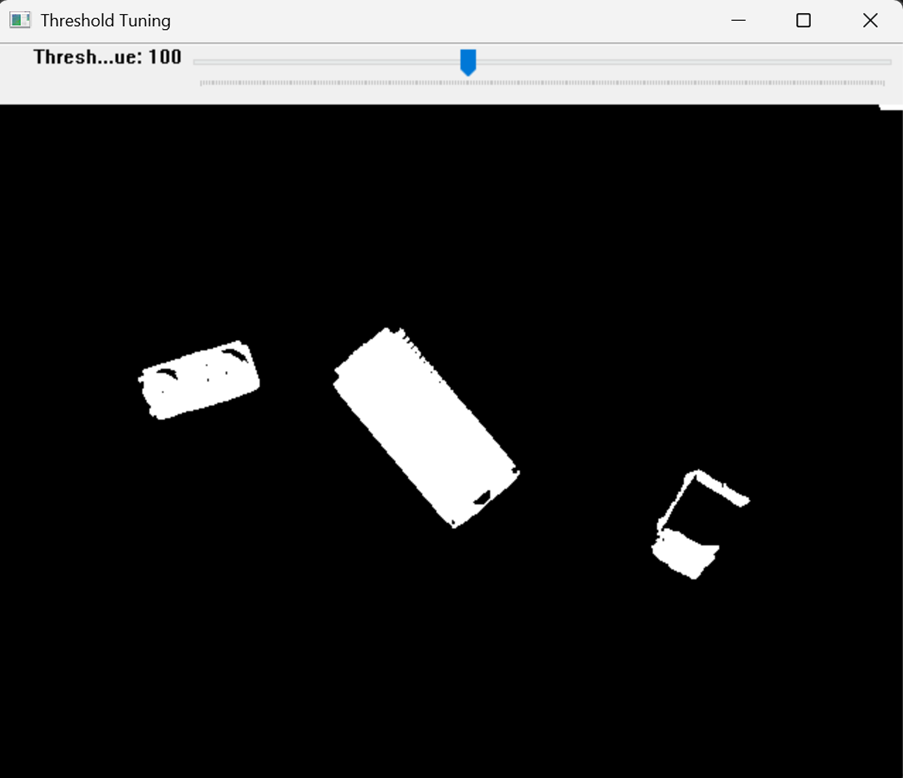
\includegraphics[width=0.78\columnwidth]{imgs/threshold_pickerbot.png}
  \caption{Image thresholding using openCV}
  \label{fig:thresholding}
\end{figure}
The machine-vision architecture is the core of the pick-and-place operation: it scans the unstructured workbench, identifies components, decodes their orientation, and translates pixel data into Cartesian coordinates for the EPSON VT6-A901S manipulator. Many industrial bin-picking solutions rely on line-of-sight 3D cameras, but these generate point clouds prone to spurious outliers on cluttered, overlapping parts, which degrade obstacle-avoidance planning and segmentation and require costly filtering \cite{Franaszek}. To avoid 3D point-cloud filtration and keep real-time processing efficient, this project uses a 2D planar overhead approach. The system developed through two phases, culminating in a deep-learning solution.

\subsubsection{Prototype Phase: Deterministic Computer Vision}
The initial architecture relied on deterministic OpenCV processing. Frames from an overhead 720p webcam were Gaussian-blurred to suppress noise, then global binary thresholding (Fig.\ref{fig:thresholding}) isolated geometric footprints. Contour analysis (\texttt{cv2.findContours}) found each object's boundary, and a scale-preserving script padded the crops into uniform 224$\times$224 tensors for a Google Teachable Machine classifier. Although functional in controlled conditions, the prototype suffered severe domain-shift failures: metallic glare erased texture, background clutter produced false ``Noise'' classifications, and axis-aligned bounding boxes could not derive the resting rotation angle (yaw).

\subsubsection{Final Architecture: YOLOv8-OBB (Oriented Bounding Box)}
\begin{figure}[t]
  \centering
  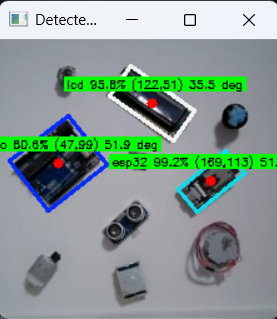
\includegraphics[width=0.78\columnwidth]{imgs/yolo_detect_v2.png}
  \caption{Image inference using yoloV8}
  \label{fig:yolo-detect}
\end{figure}
To overcome these limitations, the system was re-architected around a YOLOv8-OBB neural network that ingests the full-resolution, uncropped camera frame, eliminating manual thresholding and cropping. Trained on a custom, heavily augmented Computer Vision Annotation Tool dataset (extreme lighting shifts and rotational variance), the OBB model bypasses glare and localized clutter (Fig.\ref{fig:yolo-detect}). The manual annotation this supervised approach requires is a known but necessary trade-off for the recognition quality and spatial accuracy that bin-picking demands \cite{Fager}. In a single forward pass it outputs a 5-D oriented tensor \texttt{(cx, cy, width, height, theta)} with multi-class probabilities (Arduino, ESP32, LCD). This is far simpler than hybrid pipelines that, for example, use YOLOv5 for top-view detection followed by an eye-in-hand FAST/BRISK feature-matching step for pose estimation \cite{Taweesoontorn}. By deriving the resting angle (theta) from a single overhead frame, the OBB architecture removes any dependence on perfect lighting or multi-step image capture.
\subsubsection{Logistics Filtering and BOQ Engine}
Once the vision system extracts each component's pixel centroid $(X,Y)$ and class label, a logistics filter operates above the frame buffer. Rather than greedily forwarding every detection to the coordinate-mapping pipeline, the orchestrator matches the detected inventory against a Bill of Quantities (BOQ), ignoring surplus components even when they are validly detected, so that only the required, correctly kitted items are passed to the spatial calibration engine for EPSON translation.


\subsection{Spatial Calibration and Coordinate Mapping}
\begin{figure}[t]
  \centering
  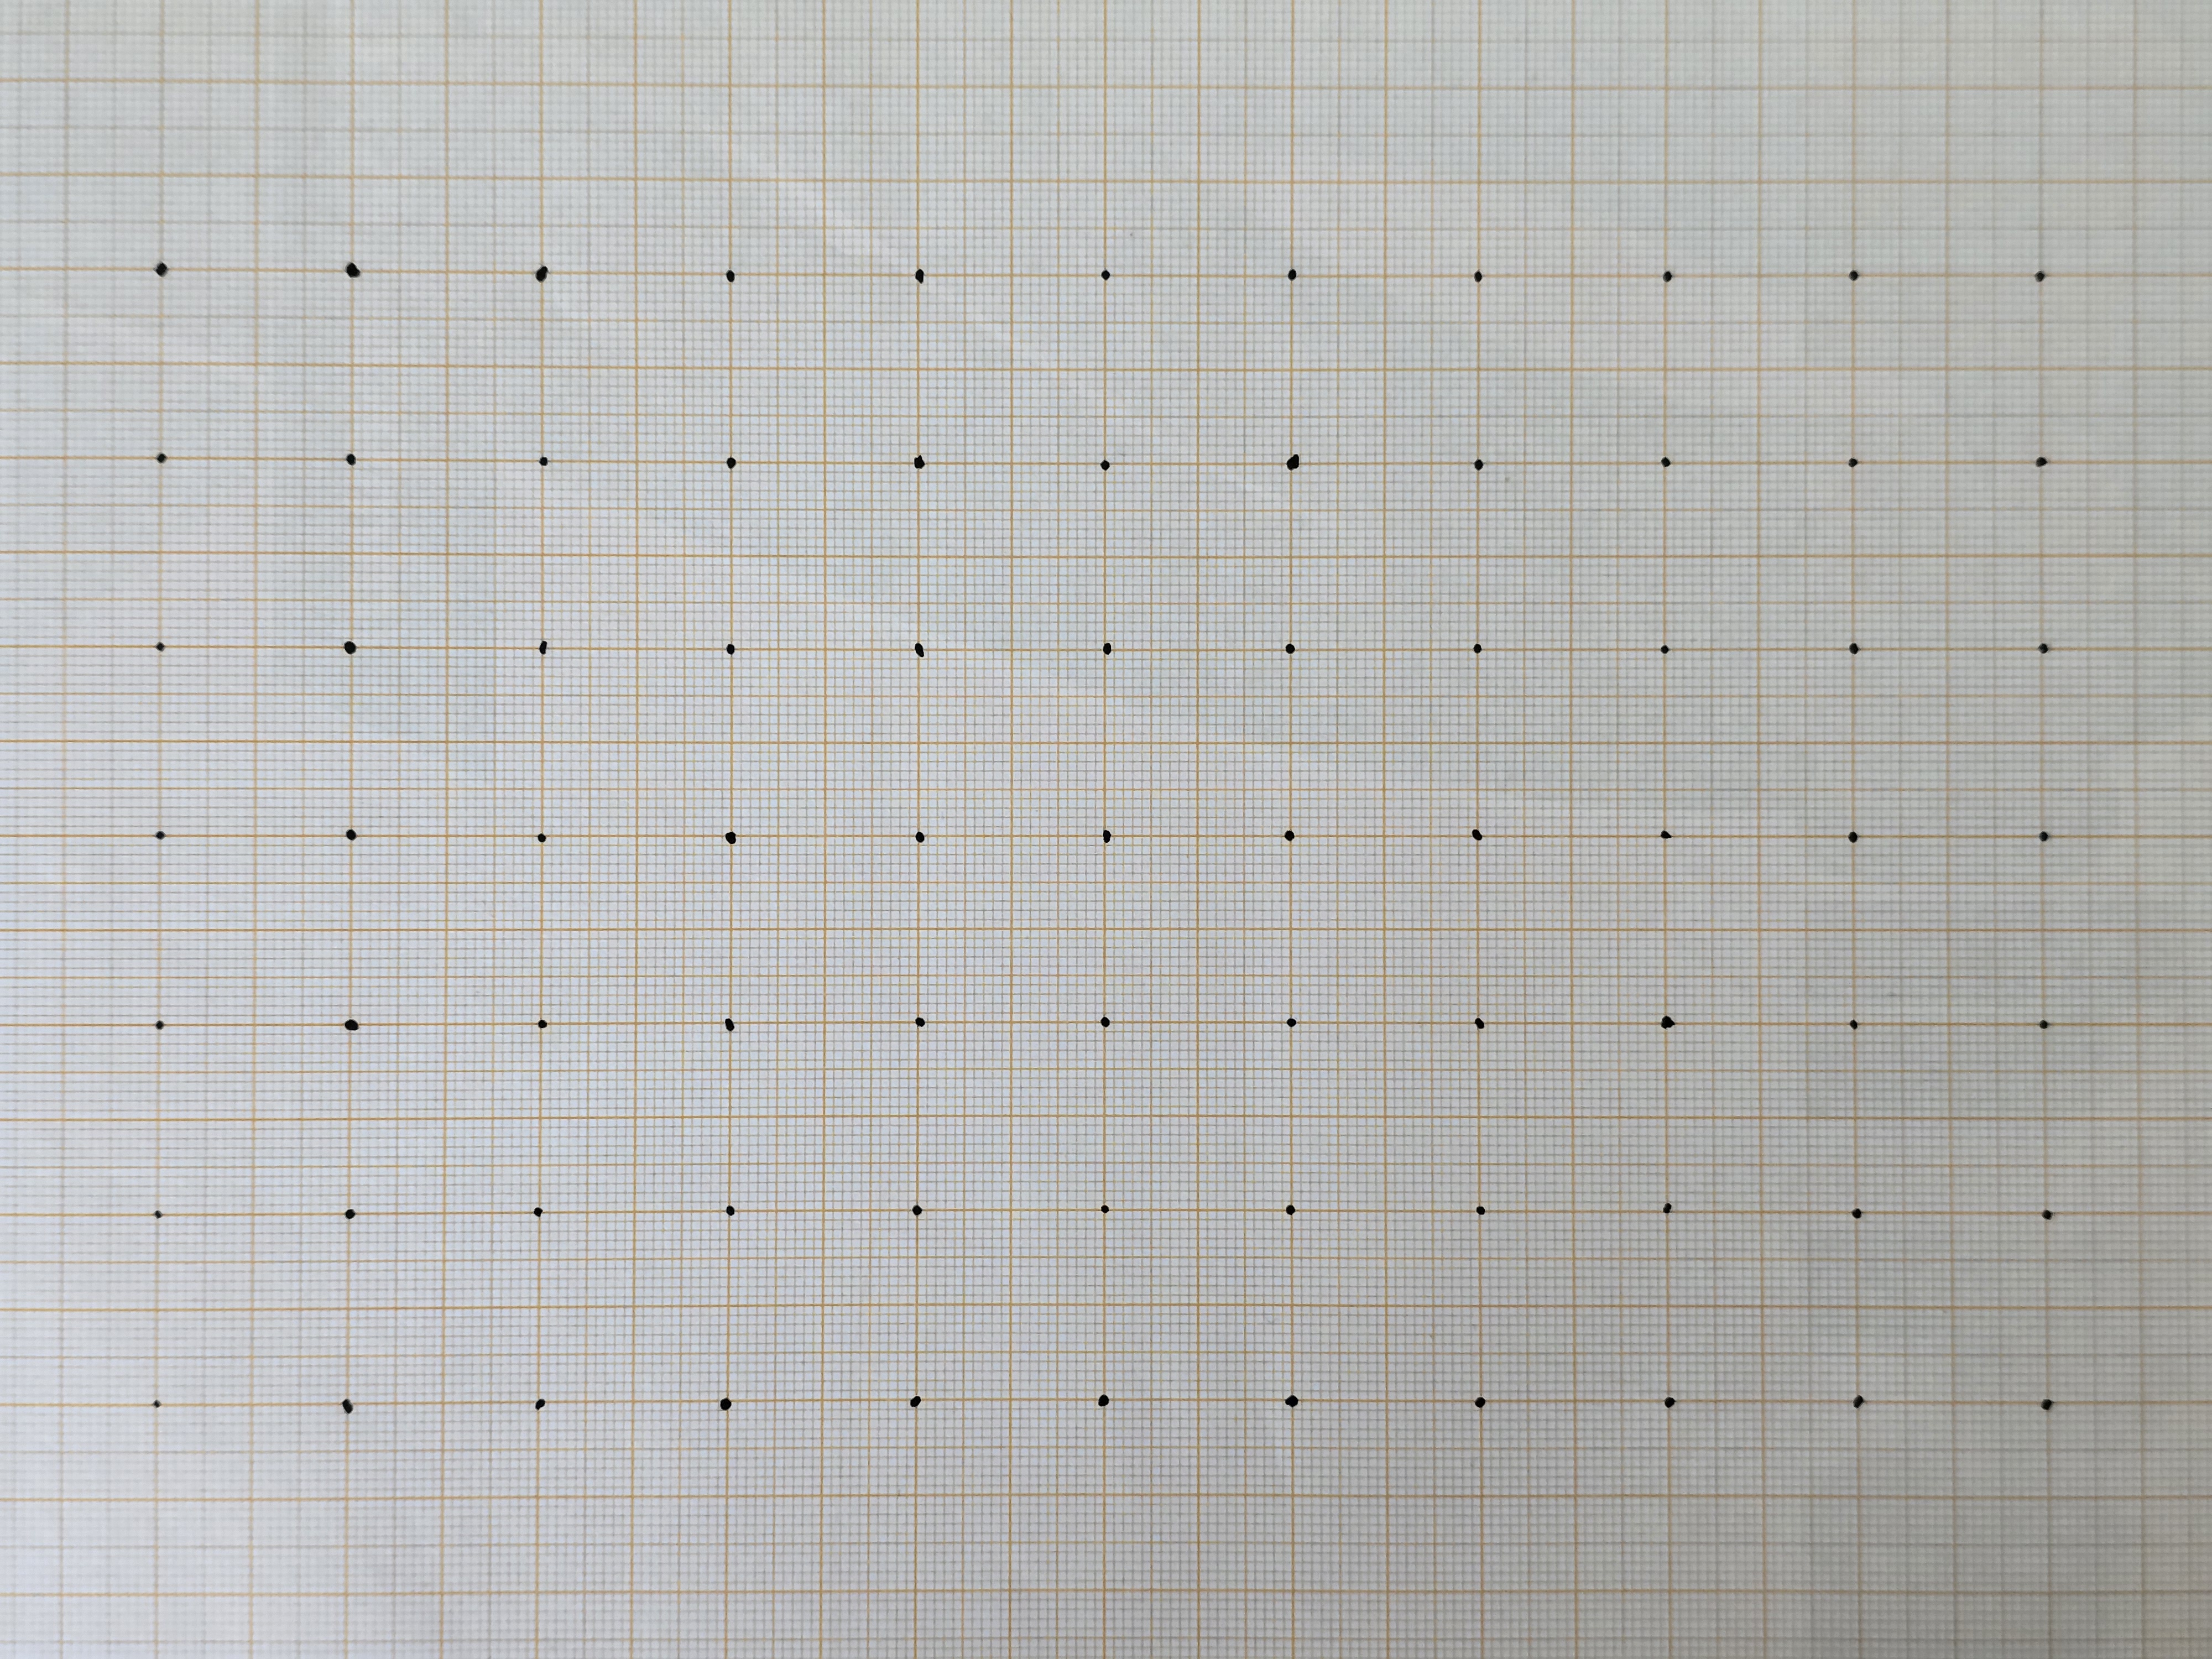
\includegraphics[width=0.78\columnwidth]{imgs/graph_paper.jpg}
  \caption{77-point homography calibration grid showing pixel click positions overlaid on the workspace reference image.}
  \label{fig:calibration_grid}
\end{figure}

A critical requirement is translating pixel positions in the camera image into physical millimetre coordinates in the robot's world frame, achieved through a planar homography that provides a projective mapping between the two coordinate spaces.

The mapping uses a 77-point calibration grid of 11 columns by 7 rows at 20~mm spacing in both axes (Fig.\ref{fig:calibration_grid}). The world X-coordinate decreases from $+$100~mm to $-$100~mm left to right and the world Y-coordinate increases from 410~mm to 530~mm top to bottom, giving a calibrated area of 200~mm $\times$ 120~mm. A reference image of the grid (\texttt{graph\_paper.jpg}) is captured with the camera normal to the workspace; \texttt{tools/calibration\_clicker.py} records the 77 intersections, and \texttt{tools/sort\_and\_tag\_pixels.py} sorts them column by column and appends the world coordinates to produce a four-column pixel-to-world CSV.

The homography matrix $\mathbf{H}$ is computed with OpenCV's \texttt{findHomography} using standard least squares (method 0), not RANSAC. This is deliberate: RANSAC rejects outliers, but the corner points define the workspace extremes and are valid, important constraints, so treating them as outliers would introduce systematic error near the boundaries. With 77 evenly distributed points, least squares gives a robust estimate without outlier rejection. At runtime, any detected centroid $(p_x, p_y)$ is mapped to world coordinates $(w_x, w_y)$ via \texttt{cv2.perspectiveTransform} with $\mathbf{H}$.

Repositioning the camera vertically changes the image scale and invalidates the pixel-to-millimetre mapping. To avoid a full recalibration, a height-recalibration routine (\texttt{pickerbot.py {-}{-}calibrate}) lets the user click two points known to be exactly 20~mm apart. Let $r_h$ and $r_v$ denote the mean pixel distance per 20~mm in the horizontal and vertical axes from the original calibration. For a measurement at angle $\theta$ to the horizontal, the expected pixel distance is the anisotropic norm:

\begin{equation}
  d_{\mathrm{expected}} = \sqrt{\left(r_h \cos\theta\right)^2 + \left(r_v \sin\theta\right)^2}
  \label{eq:expected_dist}
\end{equation}

where $\theta = \arctan2(|\Delta y|,\, |\Delta x|)$. The scale factor is then:

\begin{equation}
  s = \frac{d_{\mathrm{measured}}}{d_{\mathrm{expected}}}
  \label{eq:scale_factor}
\end{equation}

This accounts for horizontal and vertical pixel densities differing due to lens geometry or non-square sampling. All 77 coordinates are scaled about the grid centre (index~38) by $s$, written to \texttt{calibration\_pixels\_scaled.csv}, and referenced in \texttt{config.json} for subsequent runs.

\subsection{TCP/IP Communication Protocol}

\begin{table}[t]
  \caption{TCP/IP Command Set}
  \label{tab:commands}
  \centering
  \begin{tabular}{@{}llp{4.2cm}c@{}}
    \toprule
    \textbf{Command} & \textbf{Parameters} & \textbf{Robot Action} & \textbf{Reply} \\
    \midrule
    \texttt{JUMP}    & x, y, z, u & Lifts 50 mm, moves to $(x, y, z{+}50)$, descends to $(x, y, z, u)$ & OK \\
    \texttt{GO}      & x, y, z    & Linear motion to $(x, y, z)$                                      & OK \\
    \texttt{MOVE}    & x, y, z    & Linear motion to $(x, y, z)$                                      & OK \\
    \texttt{PICK}    & x, y, z, u & Full pick-and-place sequence (Section~\ref{sec:epson})             & OK \\
    \texttt{STANDBY} & ---        & Returns to home position                                           & OK \\
    \bottomrule
  \end{tabular}
\end{table}

Table~\ref{tab:commands} summarises the full command set supported by the system.

The Python control system communicates with the EPSON RC8 controller over a local TCP socket. For simulation the target is \texttt{127.0.0.1} on port 2001; for the physical robot the address is changed to \texttt{192.168.X.Y} via \texttt{config.json}. Connection management and dispatch are handled by \texttt{pickerbot\_lib.sender}, which holds a module-level socket for the session.

Commands are plain ASCII strings of the form \texttt{COMMAND~X~Y~Z~U\textbackslash r\textbackslash n}, where $X,Y,Z$ are world coordinates in millimetres and $U$ is the tool rotation in degrees. The controller replies \texttt{"OK"} after each command, and a small inter-command delay allows mechanical completion before the next is sent.

For multi-component picks, \texttt{epsonPickAll} iterates over a list of world-coordinate strings and issues a \texttt{PICK} for each, checking the reply against \texttt{"OK"}. Any non-OK response aborts the batch immediately and returns the robot to standby, so a partial failure such as a grip error or controller fault cannot leave the robot operating in an undefined state.

\begin{figure}[t]
  \centering
  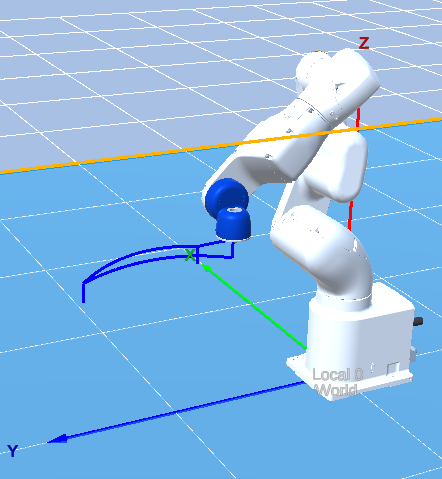
\includegraphics[width=0.8\columnwidth]{imgs/pick_trajectory.png}
  \caption{Trajectory of the \texttt{PICK} command: three-phase Jump3 approach to the component, gripper activation, transport to \texttt{PlacePoint}, and release.}
  \label{fig:pick_trajectory}
\end{figure}

Fig.\ref{fig:pick_trajectory} shows a sample pick-and-place: from standby, the arm approaches the object in the correct orientation, picks it, jumps to the place point, fixes orientation, places, and retracts to standby for the next operation.

\subsection{EPSON RC8 Robot Program}
\label{sec:epson}

The robot-side program (\texttt{Epson/Pickerbot\_Receiver/Main.prg}) is written in Epson SPEL+, the RC8 controller's scripting language, building on a template script \cite{prasetyo2024} with predefined motion-initialization parameters. After initialization it opens a TCP server on channel \#201 at port 2001 and waits for a client before entering its command loop.

Each string is split on spaces into the command token and floating-point coordinate arguments. The \texttt{PICK} command is the most complex: a three-phase Jump3 trajectory lifts the arm vertically, translates to an elevated waypoint above $(x, y)$ with the tool at orientation $u$, and descends to the pick position, where a digital output closes the gripper and a dwell ensures a reliable grip. A second Jump3 lifts clear and transports the component to a predefined \texttt{PlacePoint} (the target kit container), where the output is deactivated to release it before the arm returns to standby.

A network error handler reopens the server socket and resumes listening rather than halting, letting the system recover from transient network interruptions without operator intervention.

\subsection{Software Architecture and Entry Points}
\begin{figure}[t]
  \centering
  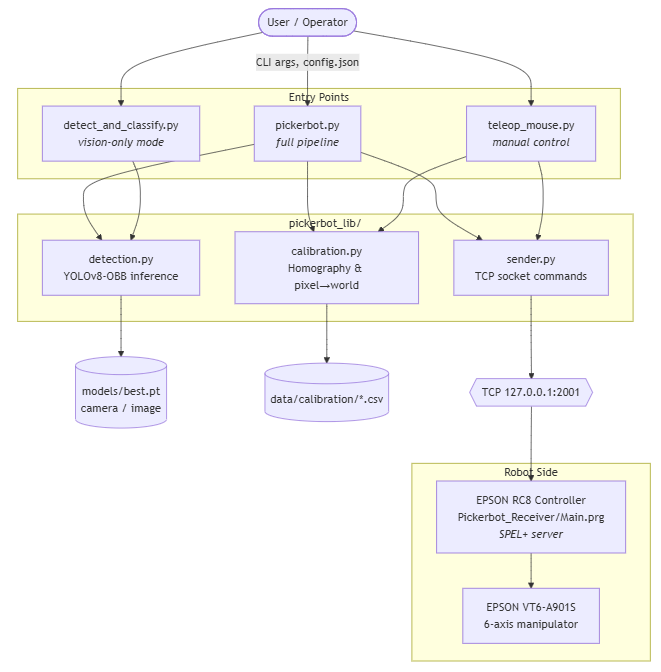
\includegraphics[width=0.85\columnwidth]{imgs/software_architecture.png}
  \caption{Software architecture of the Picker-Bot system, illustrating the three entry-point scripts and their shared dependency on the \texttt{pickerbot\_lib} package.}
  \label{fig:architecture}
\end{figure}

The codebase (Fig.\ref{fig:architecture}) is built around a shared package, \texttt{pickerbot\_lib}, consolidating detection, calibration, and TCP communication into three submodules: \texttt{detection}, \texttt{calibration}, and \texttt{sender}. Three entry-point scripts at the project root each import this package to serve a distinct mode.

The primary entry point, \texttt{pickerbot.py}, orchestrates an end-to-end pick session. A \texttt{{-}{-}src} argument selects the detection source (live camera or a static image), and \texttt{{-}{-}calibrate} launches the height-recalibration GUI and exits. In a normal run it loads the homography CSV named in \texttt{config.json}, runs detection to obtain centroid pixels, maps each to world coordinates, and dispatches the list to \texttt{epsonPickAll} over TCP.

The second, \texttt{detect\_and\_classify.py}, isolates the vision layer for development and testing without a robot connection: given a file path it processes a static image, and without arguments it opens the live feed with a real-time confidence-threshold slider.

The third, \texttt{teleop\_mouse.py}, provides interactive positioning: it loads the calibration, connects to the robot, and displays the reference image with all 77 points annotated. Each click is transformed through $\mathbf{H}$ and sent as a \texttt{MOVE} command, enabling manual positioning without the full pipeline, which is useful for verifying calibration accuracy before an automated session.

\subsection{Robotic Control and Simulation}
Manipulation is simulated in the EPSON RC8.0 environment. The system can cover any workspace size; the initial setup mapped a 200~mm $\times$ 120~mm evaluation space with a deposit point 280~mm above its centre. The platform is the EPSON VT6-A901S~\cite{b2}, a 6-axis arm with 980~mm reach suited to pick-and-place requiring varied approach angles and high repeatability; full installation, safety, and operational specifications appear in the Epson VT6 documentation \cite{epsonvt6}.
\section{Results}
The Picker-Bot system integrated deep-learning vision with industrial robotic control inside the EPSON RC8.0 simulator. The following subsections report observed behaviour across three layers: perception, spatial reasoning, and supervised manipulation.

\subsection{Vision System Performance and Robustness}
\begin{figure}[t]
    \centering
    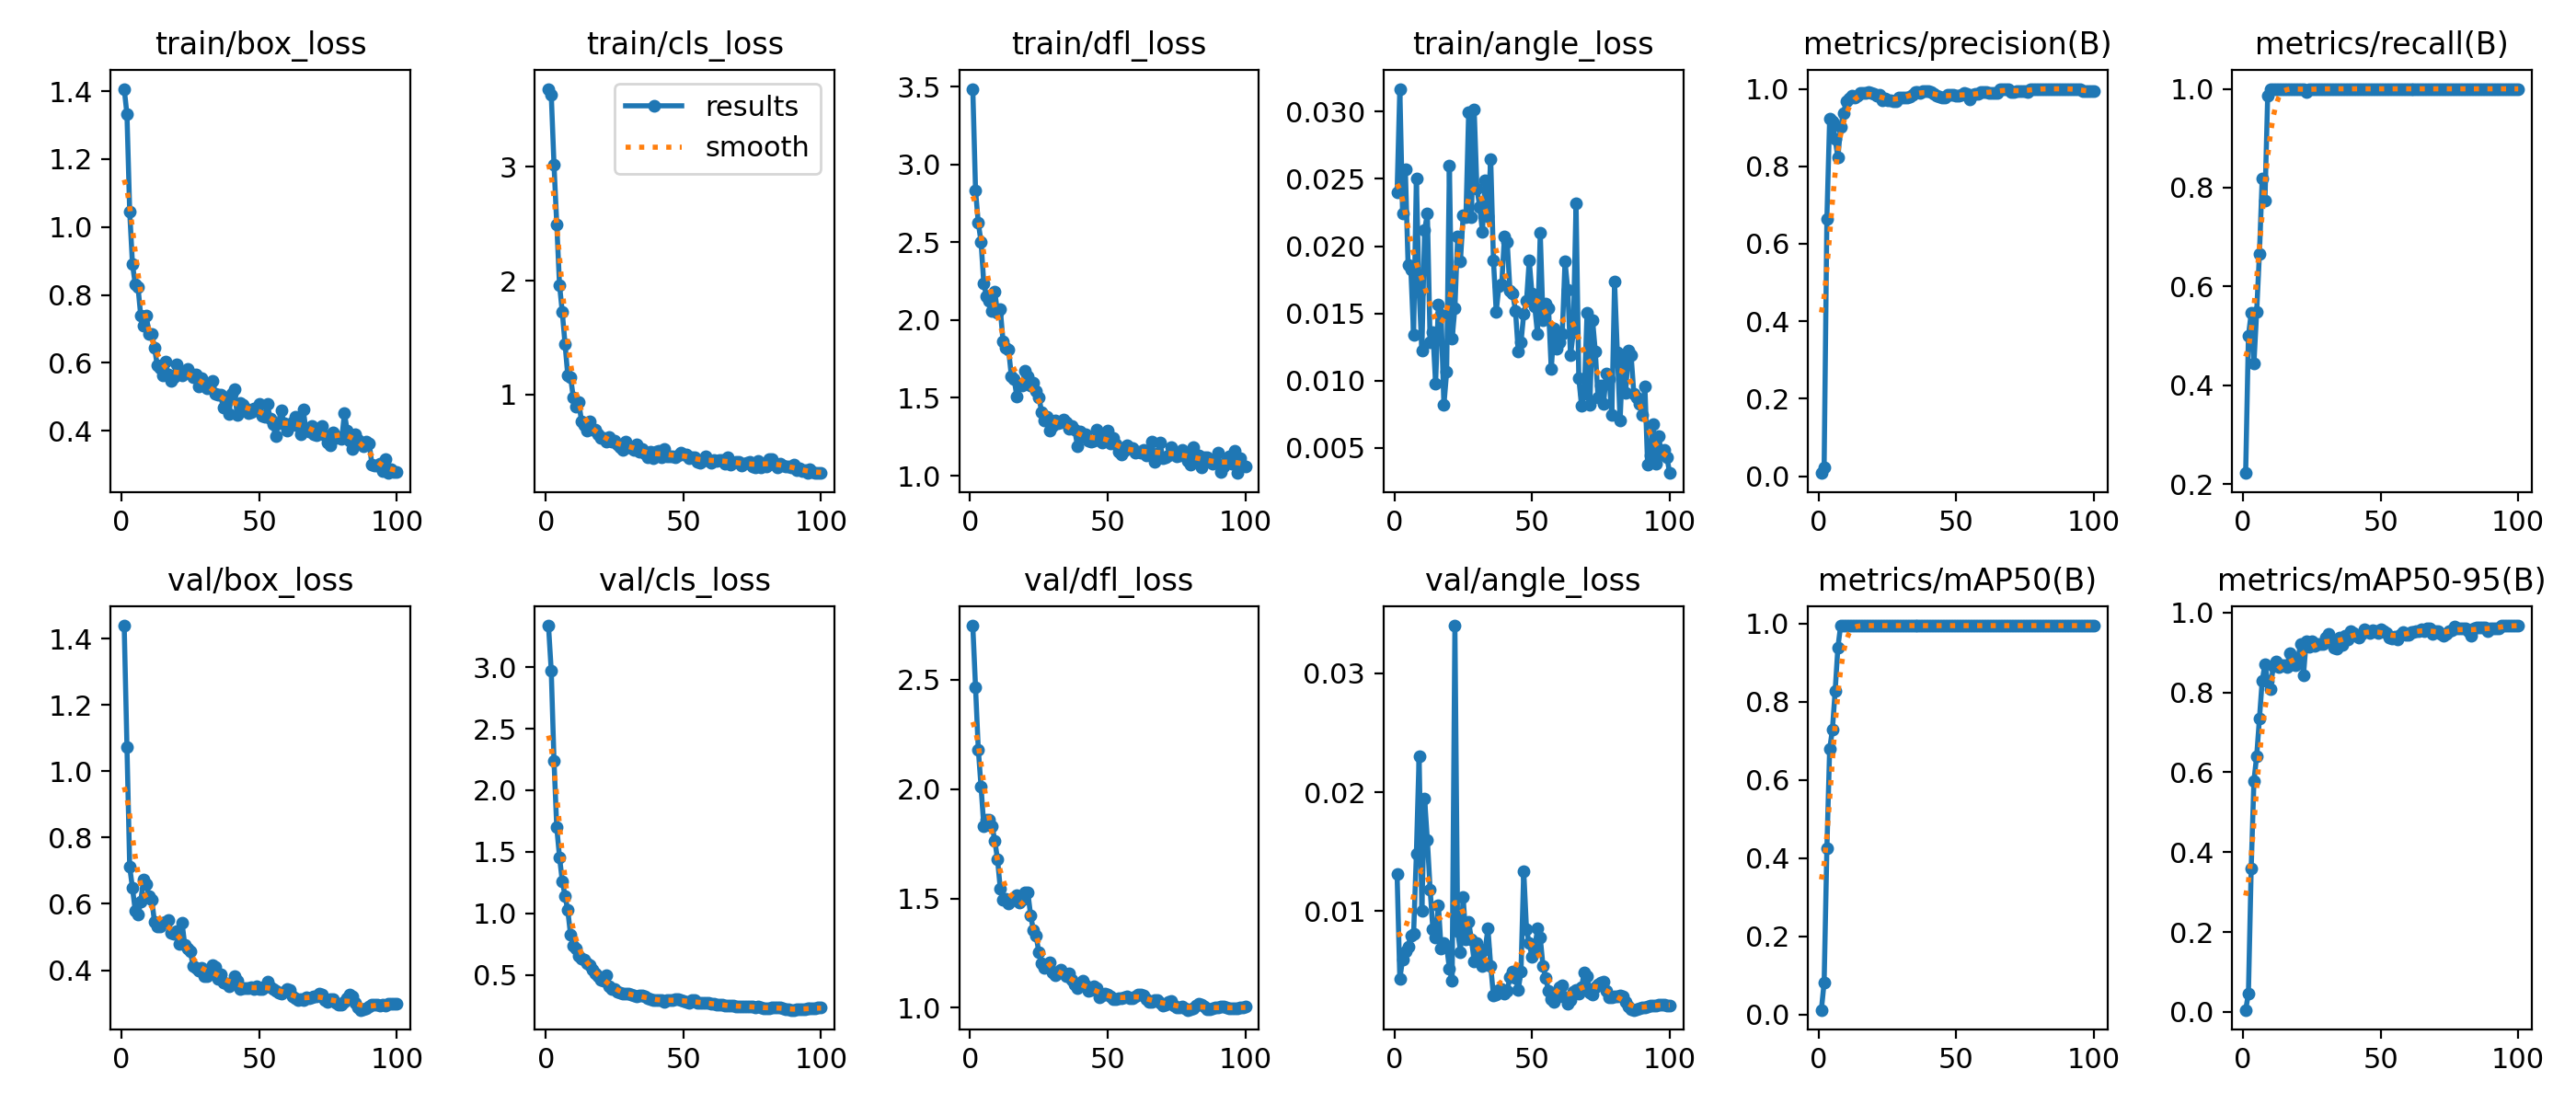
\includegraphics[width=0.85\columnwidth]{imgs/yolo_results.png}
    \caption{YOLOv8-OBB training metrics. Loss curves and $mAP_{50}$ progression demonstrating rapid convergence and high detection accuracy on the in-distribution component set.}
    \label{fig:yolo_results}
\end{figure}

The migration from the OpenCV prototype to the YOLOv8-OBB architecture substantially improved detection reliability. The final model classified Arduino, ESP32, and LCD modules and recovered the resting angle $\theta$ with the centroid $(cx, cy)$ in a single forward pass, with no geometric post-processing, and absorbed the glare, clutter, and background texture that had destabilised the prototype. An explicitly trained ``noise'' class was suppressed at the output, so only valid components reached the coordinate-mapping layer.

Fig.~\ref{fig:yolo_results} plots the training loss and mean Average Precision: the model converged rapidly to a final $mAP_{50}$ of 0.99, indicating near-perfect localisation and classification within the training distribution. A fixed confidence threshold of 0.7 eliminated the few remaining glare-induced false positives, with no additional non-maximum suppression required.

\subsection{Spatial Calibration and Mapping Accuracy}
The homography reliably bridged the camera image and the planar workspace, with the 77-point grid defining a calibrated region of roughly $200~\text{mm} \times 120~\text{mm}$ that covered the full overhead field of view. Using least squares rather than RANSAC kept the boundary corner points from being discarded as outliers, which would otherwise have contracted the calibrated area.

Height recalibration absorbed camera repositioning in seconds without re-clicking every intersection: measuring a known 20~mm segment against the original grid pitches recovered an anisotropic scale factor applied about the grid centre. The result was verified through \texttt{teleop\_mouse.py}, where each click produced a \texttt{MOVE} command whose terminal position visually matched the clicked feature.

\subsection{Integrated Robot Control and Logistics}
The control pipeline exercised the pull-based kitting end-to-end. Given a BOQ, the system satisfied its requirements in order of detection confidence and ignored correctly recognised but unneeded components, behaving as a logistics auditor rather than a greedy collector; without a BOQ it reverted to greedily picking every non-noise detection.

The TCP/IP interface dispatched the full command set (\texttt{JUMP}, \texttt{GO}, \texttt{MOVE}, \texttt{PICK}, \texttt{STANDBY}) reliably across extended runs, each validated by an \texttt{OK} reply before the next was sent. The \texttt{PICK} primitive executed its three-phase Jump3 trajectory in every trial, and synthetic failures exercised the abort path, returning the manipulator to standby rather than continuing through an undefined state. Across all configurations the system switched cleanly between live USB and pre-recorded images via a single \texttt{config.json} setting, interfaced with the RC8.0 simulator at \texttt{127.0.0.1}, and kept 0.7 as the default confidence threshold while exposing a runtime slider.
\section{Future Discussion}
The current implementation demonstrates the concept in simulation; several avenues remain for further development.

The most immediate step is deployment to physical hardware. Moving from the RC8.0 simulator to a real VT6-A901S will require calibrating the physical camera under varying lighting and tuning gripper timing to the mechanical characteristics of real components; handling delicate modules of varying shape and mass may also require an adaptive or compliant gripper to avoid damage.

Further ahead, a web-based portal would let students and staff submit BOQs directly; the system could queue requests, process inventory overnight, and notify users when a kit is ready, making recovery self-service and reducing staff workload. To automate the physical logistics of the pull model, future iterations could integrate Internet of Things (IoT) technologies and Autonomous Guided Vehicles (AGVs), increasingly used in flexible manufacturing to route materials across facilities \cite{vlachos}: an IoT-guided AGV network could fetch bins of returned kits to the workcell and deliver finished kits to student collection points.

\section{Conclusion and Discussion}
\subsection{Critical Evaluation of System Integration}
The Picker-Bot system successfully shifted component kitting from a ``push'' model to a project-specific ``pull'' model. Its technical cornerstone was the migration from deterministic OpenCV prototypes to YOLOv8-OBB: where the prototype was highly sensitive to environmental shifts, the final model reached a $mAP_{50}$ of 0.99, showing that high-accuracy bin-picking is viable in cluttered educational settings without 3D point-cloud hardware. The ``logistics auditor'' approach---filtering detections through the BOQ engine---lets the system both detect parts and manage inventory, directly addressing the goal of reducing procurement costs and e-waste.
\subsection{Implementation Constraints and Real-World Considerations}
Several constraints would affect any physical deployment. The fixed software delay after each \texttt{OK} kept the simulated pipeline stable but should instead be tuned to each component's inertia, since a heavier LCD settles differently from a lighter ESP32 and a single value trades throughput against reliability. The 77-point homography is a planar model of a three-dimensional problem: components of non-negligible height introduce a parallax offset that appears as a small systematic lateral error during the Jump3 descent, so a height-aware correction (per-class offsets or a depth sensor) would be needed. Finally, the abort-on-failure strategy---correct as an industrial default---is blunt at higher throughputs, where a graduated model distinguishing transient communication faults from genuine mechanical errors would be necessary to scale to production volumes.
\subsection{Concluding Remarks}
In conclusion, the Picker-Bot system provides a technically sound, sustainable solution for managing returned educational circuit kits. By integrating Oriented Bounding Box detection, planar homography, and TCP/IP control, it shows that modern AI can turn ``loose waste'' into project-ready assets, setting a precedent for ``Re-X'' (Recovery and Re-use) activities in microelectronic environments and bridging waste management with logistical efficiency.
\section*{Acknowledgment}
The authors acknowledge the guidance and resources of the PDE4435 module, which encouraged a design-thinking approach to advanced robotics projects, and the use of Claude during project development.

\begin{thebibliography}{00}
\bibitem{amp}
AMP, ``AMP ONE: Automated Waste Sorting Systems \& Facility,'' 2026. [Online]. Available: \url{https://ampsortation.com/products/amp-one}.
\bibitem{saenz}
J. Saenz \textit{et al.}, ``Automated disassembly of e-waste---requirements on modeling of processes and product states,'' \textit{Frontiers in Robotics and AI}, vol. 11, p. 1303279, 2024.
\bibitem{Franaszek}
M. Franaszek, P. Rachakonda, and K. S. Saidi, ``Filtering Organized 3D Point Clouds for Bin Picking Applications,'' \textit{Applied Sciences}, vol. 14, no. 3, p. 961, Jan. 2024.
\bibitem{Fager}
P. Fager, R. Hanson, \text{\AA}. Fasth-Berglund, and S. Ekered, ``Supervised and unsupervised learning in vision-guided robotic bin picking applications for mixed-model assembly,'' \textit{Procedia CIRP}, vol. 104, pp. 1304--1309, 2021.
\bibitem{Taweesoontorn}
T. Taweesoontorn, S. Yanyong, and P. Konghuayrob, ``Hybrid Deep Learning and FAST--BRISK 3D Object Detection Technique for Bin-picking Application,'' \textit{Sensors and Materials}, vol. 36, no. 4, pp. 1389--1404, 2024.
\bibitem{prasetyo2024}
J. Prasetyo, ``RC7\_Python,'' Jan. 03, 2024. Available: \url{https://github.com/judhi/RC7_Python}.
\bibitem{b2} EPSON Robotics, ``RC8.0 Reference Manual,'' EPSON Factory Automation, 2023. [Online]. Available: https://www.epson.com
\bibitem{epsonvt6}
Epson America, Inc., ``Epson VT6L All-in-One 6-Axis Robots | Support,'' Epson US, 2026. [Online]. Available: \url{https://epson.com/Support/Robots/6-Axis-Robots/VT-Series/Epson-VT6L-All-in-One-6-Axis-Robots/s/SPT_VT6L-A901SS}.
\bibitem{vlachos}
I. Vlachos, R. M. Pascazzi, M. Ntotis, K. Spanaki, S. Despoudi, and P. Repoussis, ``Smart and flexible manufacturing systems using Autonomous Guided Vehicles (AGVs) and the Internet of Things (IoT),'' \textit{International Journal of Production Research}, pp. 1--22, 2022.
\end{thebibliography}

\end{document}
